%\documentclass[12pt,a4paper,twoside]{article}    % 
\documentclass[times]{fldauth}
\usepackage{graphicx,multicol,color,footmisc} % Packages for svmult %   
\usepackage{amssymb,amsthm,amsmath}
\usepackage{psfrag}
%\usepackage[numbers]{natbib}% Literaturzitate mit Autor und Jahr im Text
\usepackage{cite} 
% definitions used by included articles, reproduced here for 
% educational benefit, and to minimize alterations needed to be made
% in developing this sample file.
\newtheorem{rem}{Remark}

%\newcommand{\Bausteine}{/home/mm/Markus/Papers/Markus/Bausteine}
\newcommand{\imsizes}{0.31\textwidth}
\newcommand{\imsizem}{0.48\textwidth}
\newcommand{\imsizel}{0.90\textwidth}
\newcommand{\imsizexl}{0.95\textwidth}
% mathematical commands
\newcommand{\pe}{\psi}
\newcommand{\mb}{\mathbf}
\newcommand{\bvh}{\mb v^h}
\newcommand{\bwh}{\mb w^h}
\newcommand{\bVh}{\mathbf V^h}
\newcommand{\pdiff}[2]{\frac{\partial#1}{\partial #2}}
%die folgenden Macros werden wegen einem Paketkonflikt zwische amstex und typedref manuell definiert
%dadurch sind keine unterstriche in labelnamen mehr möglich
\newcommand{\sectionref}[1]{Section \ref{#1}}
\newcommand{\figureref}[1]{Fig. \ref{#1}}
%\newcommand{\eqref}[1]{(\ref{#1})}
\newcommand{\chapterref}[1]{chapter \ref{#1}}
\newcommand{\lemmaref}[1]{Lemma \ref{#1}}
\newcommand{\tableref}[1]{\ref{#1}}
\newtheorem{lemma}{Lemma}[section]
\def\d{\delta} 
\def\ds{\displaystyle} 
\def\e{{\epsilon}} 
\def\eb{\bar{\eta}}  
\def\enorm#1{\|#1\|_2} 
\def\Fp{F^\prime}  
\def\fishpack{{FISHPACK}} 
\def\fortran{{FORTRAN}} 
\def\gmres{{GMRES}} 
\def\gmresm{{\rm GMRES($m$)}} 
\def\Kc{{\cal K}} 
\def\norm#1{\|#1\|} 
\def\wb{{\bar w}} 
\def\zb{{\bar z}} 

% some definitions of bold math italics to make typing easier.
% They are used in the corollary.

\def\bfE{\mbox{\boldmath$E$}}
\def\bfG{\mbox{\boldmath$G$}}

\title{Stabilization of the 3-D spherical convection code Terra}

% The thanks line in the title should be filled in if there is
% any support acknowledgement for the overall work to be included
% This \thanks is also used for the received by date info, but
% authors are not expected to provide this.

\author{Markus M\"uller, Christoph K\"ostler}

\begin{document}

\maketitle

\begin{abstract}
We apply the stabilization technique of Dohrmann, Bochev and Gunzburger 
%\cite{Dohrmann2004} 
to the 3-D widely used spherical mantle convection simulation code Terra by John Baumgardner.
%\cite{Baumgardner1985},
The latter uses an equal-order finite-element discretization, which is not inf-sup stable.
Following the original approach, a stabilization matrix representing a projection operator is introduced.
Whereas the implementation of the stabilization has been straight forward, it remains to show that its stability
actually can be proved in the more general situation arising  from the nonstandard finite elements used in the code.
Numerical experiments with the improved solver show that the method works in praxis. 
\end{abstract}

%\begin{keywords} 
 \keywords{  inf-sup, stabilization, equal-order discretization, finite elements,mantle convection}
%\end{keywords}

%\begin{AMS}
%15A15, 15A09, 15A23
%\end{AMS}

%\pagestyle{myheadings}
%\thispagestyle{plain}
%\markboth{TEX PRODUCTION AND V. A. U. THORS}{SIAM MACRO EXAMPLES}

%%%%%%%%%%%%%%%%%%%%%%%%%%%%%%%%%%%%%%%%%%%%%%%%%%%%%%%%%%%%
\section{Introduction}
%%%%%%%%%%%%%%%%%%%%%%%%%%%%%%%%%%%%%%%%%%%%%%%%%%%%%%%%%%%%
We first shortly describe the application range of our simulation code as 
it broadened during its development - using numerical improvements and imposing new challenges - 
and then compare it to present day alternative approaches from a numerical point of view. 
We then outline the technical improvements described in the paper. 
%%%%%%%%%%%%%%%%%%%%%%%%%%%%%%%%%%%%%%%%%%%%%%%%%%%%%%%%%%%%
\subsection{Modeling Convection and Evolution of the Earth's Mantle Using Terra}
%%%%%%%%%%%%%%%%%%%%%%%%%%%%%%%%%%%%%%%%%%%%%%%%%%%%%%%%%%%%
One of the earliest three-dimensional numerical models of mantle convection was the 
spherical-shell model Terra, developed by John Baumgardner \cite{Baumgardner1983,Baumgardner1985a}.
It uses a finite-element discretization on a pentahedral grid (prisms with spherical triangles as top and bottom faces), and it utilizes
an efficient multigrid algorithm to solve for the velocity. 
It was parallelized by Bunge and Baumgardner \cite{Bunge1995} through message passing and
lateral domain decomposition in two of three dimensions. A first study of
convection with Earth-like Rayleigh number of $10^8$ and depth-dependent
viscosity was done by Bunge, Richards and Baumgardner \cite{Bunge1997}. 
At the same time, Yang \cite{Yang1997}
improved the multigrid algorithm with matrix-dependent transfer operators to
represent varying viscosity properly . With this code,
Richards \cite{Richards2001} investigated surface mobility as a function of viscosity
variation and yield stress, and Reese \cite{Reese2005} explored a parameter range of 
$\Delta \eta$ between $10^5$ and $5 \times 10^7$ with an internal Rayleigh
number of $10^6$. Based on postglacial rebound, mantle mineralogy, seismic tomography, 
thermodynamics and high-pressure geophysics, Walzer \cite{Walzer2004a} derived a viscosity profile with three
high-viscosity and three low-viscosity zones and steep gradients.
Even though this  model  had to be restricted especially regarding lateral variations of viscosity 
due to temperature-dependence, which it has not yet been possible to resolve numerically,
they were able to reproduce the evolution of self-consistent oceanic plates 
in connection with the thermal evolution of the the Earth. 
More recently Walzer \cite{Walzer2008a,Walzer2008b} showed the importance of these viscosity
variations for plate tectonics and surface mobility on Earth and incorporated
chemical differentiation of continents and, as a complement, of the
depleted MORB mantle (DMM). In their model, continents evolve by the interplay
of chemical differentiation and convection/mixing, without the requirement
of modified boundary conditions on the outer surface of the shell. DMM is partly
stirred into the other mantle reservoirs, resulting in a marble-cake mantle with
a high concentration of DMM in the asthenosphere \cite{Walzer2011}.
Terra was also applied by Oldham \cite{Oldham2004} to investigate layered convection 
and by Bunge and Davies \cite{Bunge2005,Davies2005a,Davies2005,Davies2009} to study thermally driven mantle plumes.
To reach a higher grid resolution in the upper mantle, Davies \cite{Davies2008} added
a multi-resolution multigrid method to Terra.

Phillips and Coltice \cite{Phillips2005,Phillips2007,Coltice2007,Phillips2009,Phillips2010} studied the influence of mobile continents on mantle temperature and convective wavelength.

Bunge \cite{Bunge2001} used Terra to calculate mantle flow in a circulation model
to further constrain seismic tomographic imaging of the mantle. 
They further did inverse modeling with data assimilation for the past 200~Ma \cite{Bunge2002,Bunge2003} 
to infer mantle flow and structure from seismic tomography and plate motion history.
Schuberth \cite{Schuberth2009,Schuberth2009a} also investigated thermal and elastic properties and heterogeneities within the mantle to explain velocity models based on global seismic tomography.

Iaffaldano \cite{Iaffaldano2007} coupled Terra to a lithospheric model to study plate coupling at the Nazca-South America
convergent margin.
%%%%%%%%%%%%%%%%%%%%%%%%%%%%%%%%%%%%%%%%%%%%%%%%%%%%%%%%%%%%
\subsection{Numerical Methods}
%%%%%%%%%%%%%%%%%%%%%%%%%%%%%%%%%%%%%%%%%%%%%%%%%%%%%%%%%%%%

Stable Stokes solvers as parts of simulations of convection in planetary mantles are not yet standard.
There is a reasonable number of codes using nearly as many numerical approaches.  
Early examples of finite difference (FD) methods are the codes of Ratcliff and Yoshida \cite{Ratcliff1995,Yoshida1999} 
which use a latitude-longitude grid.
%However, as their grid lines converge at the poles, they pose heavy constraints on the time step length.
%
Many other FD models connect several patches of nearly orthogonal grids to a global spherical grid, either non-overlapping 
%\cite{Zhong2000,Zhong2007a,Burstedde2009} 
\cite{Zhong2000,Zhong2007a} 
or even overlapping patches \cite{Yoshida2006,Tackley2008}.
%
Some \cite{Harder2005,Stemmer2006} use finite volume (FV) approaches.
%
Beside our own model \cite{Baumgardner1985,Baumgardner1985a} some other codes \cite{Zhong2007a,Burstedde2009} use finite elements (FE).

While it is hopeless to try to prove numerical stability for the different FD approaches, theory exists to handle the FV and FE cases.
%
However, whereas the FV methods mentioned above are proved to be stable by the theory, this is not true for most of the FE approaches which \emph{all} use unstable finite element pairs.

Although the violation of the LBB stability condition by low-order velocity-pressure pairs has been known since 1974 \cite{Brezzi1974existence},
they still have been the method of choice for many applications.
Their attraction arising from the simple data structures, the moderate size of the arising algebraic problems and low bandwidth even in three dimensions
often seems to compensate the additional effort generated by the need to stabilize the arising linear systems subsequently or post-process the data.
Fortunately, the question of stability has recently gained attention from the mantle-convection community so that the need for stabilization is eventually addressed. 
Accordingly, \cite{Burstedde2009} who use a unstable $Q_1-Q_1$ discretization apply a polynomial pressure stabilization.
Another available and widely used FE code \cite{Zhong2007a} still uses an unstabilized $Q_1-P_0$ discretization and tries to circumvent some of the effects of it's inf-sup deficiency with a penalty method.
The same verdict unfortunately holds for the Terra code we have been using for several years.
There is no proof of its stability for the Stokes system, which is furthermore not to be expected for the basic finite element pair since an equal-order interpolation is used. 

This paper describes how this shortcoming is repaired with a stabilization method. 
A brief overview of the variety of availabe stabilization approaches including a new one is given in \cite{bochev2007stabilization}, a more detailed in \cite{barth2004taxonomy}.
The new approach is appealing because it requires neither the computation of derivatives, mesh-dependent parameters nor the introduction of nonstandard data structures and leads to symmetric matrices. 
These properties render it very appropriate for the implementation in an already existing code.
%
However, there is one obstacle to overcome which consists in the nonstandard FE defined on Terra's nonstandard grid.   
The latter is based on an icosa\-hedral triangulation of the sphere \cite{Baumgardner1985,Baumgardner1985a} (see \ref{sec:grid}). 
The same grid is also widely used in oceano\-graphy \cite{Boal2008} and weather forecast \cite{Randall2002} and is well suited to finite elements.

The remainder of the paper proves that it also meets the requirements of the stabilization method  \cite{bochev2007stabilization} and is structured as follows:
In \sectionref{sec:nom} we  give a brief overview of the used finite element spaces and the nomenclature used throughout the paper.
The material needed to show the desired stability is presented in  \sectionref{chap:prevres}.
The proof of stability will be given in \sectionref{sec:proof}.
In \sectionref{chap:outline} we outline the essential steps according to \cite{bochev2007stabilization} and mark the alterations to essential lemmata
required by our 3-D spherical elements whose proofs will be subsequently given in \chapterref{chap:terralemmata}.



%%%%%%%%%%%%%%%%%%%%%%%%%%%%%%%%%%%%%%%%%%%%%%%%%%%%%%%%%%%%
\subsection{Governing Equations}
%%%%%%%%%%%%%%%%%%%%%%%%%%%%%%%%%%%%%%%%%%%%%%%%%%%%%%%%%%%%
The mathematical formulation of convection in the Earth's mantle consists of a
(generalized) Stokes equation system for velocity and pressure, supplemented by an
energy equation, an equation of state and a set of boundary conditions. 
With respect to stability we only consider the Stokes system. 
It comprises the conservation equations for momentum and mass.
\begin{eqnarray}
   - \nabla \cdot \tau + \nabla p &=& \rho \mb g \label{eq:momentum} \\ 
   \pdiff{\rho}{t} + \nabla \cdot(\rho \mb u) &=& 0, \label{eq:mass} 
\end{eqnarray}
where $\mb u$ is the velocity, $p$ pressure, $\rho$ density, 
$\mb g$ gravity and $\tau$ the deviatoric shear stress tensor. 
In the momentum equation (\ref{eq:momentum}), $\mb u$ is included implicitly
through $\tau$. 

Most regions of the mantle are characterized by linear rheology, thus it is a special case of the model.
Then the stress tensor is related to strain rate, $\dot\varepsilon$, by
\begin{eqnarray}
   \tau_{lm} &=& 2\eta\left(
	 \dot\varepsilon_{lm} - \frac{1}{3}\delta_{lm}\dot\varepsilon_{kk}
	 \right) \\
      &=&  \eta\left( \pdiff{u_l}{x_m} + \pdiff{u_m}{x_l} 
	 - \frac{2}{3} \delta_{lm}\pdiff{u_k}{x_k} \right), \label{eq:tau} 
\end{eqnarray}
where $\eta$ is the dynamic shear viscosity. 
Because density variations are rather small on a local scale, many models use the Boussinesq-approximation. 
Then the third summand in (\ref{eq:tau}) 
vanishes, leading to:
%,leading to:
\begin{equation}
   \tau_{lm} = \eta \left(\pdiff{u_l}{x_m} + \pdiff{u_m}{x_l}\right).
   \label{eq:tau_inc} 
\end{equation}
Then, with $\rho=const$, the mass equation (\ref{eq:mass}) simplifies to:
\begin{equation}
   \nabla \cdot  u = 0  \label{eq:mass_inc} 
\end{equation}
The last simplification justifies the common operator notation:
\begin{eqnarray*}
A \mb u + B^T p 	&=& 	\mb f \\
          B \mb u	&=&	0
\end{eqnarray*}
In regard to boundary conditions we restrict ourselves here to the Dirichlet case since our main focus is stability with respect to the grid. 
It should be mentioned that some of the realistic boundary conditions for mantle convection simulations as e.g. the free slip condition on the spherical surfaces involve additional inf-sup conditions \cite{Finite_element_approximation_of_incompressible_Navier_Stokes_equations_with_slip_boundary_condition,Finite_element_approximation_of_incompressible_Navier_Stokes_equations_with_slip_boundary_condition_II}.
We also mention that a more detailed analysis of a spatially dependent density further complicates the situation considerably \cite{bernardi_Finite_Element_Approximation_of_Viscous_Flows_with_Varying_Density} even for standard Dirichlet boundary conditions, let alone the more general situation mentioned above. 
We also do not consider the from a practical point of view very interesting case of spatially varying viscosity explicitly although the theory is probably applicable without much further difficulties. 
We mention \cite{Tabata2000,Tabata2002,Tabata2006} as an example where a continuously differentiable spatially viscosity has been successfully integrated in the theoretical framework.
The attempt of a stability proof is however hopeless if the viscosity depends on (dynamic) pressure or nonlinearly on velocity.
We cannot consider these general cases here, but try to establish stability at least for the  Stokes system, since this is nowadays fortunately considered a fundamental requirement for 
\emph{any} convection code, e.g. to compute intermediate results correctly that arise from the linearizations of those more realistic models.  
%%%%%%%%%%%%%%%%%%%%%%%%%%%%%%%%%%%%%%%%%%%%%%%%%%%%%%%%%%%%
\subsection{Terra's Grid}
\label{sec:grid}
%%%%%%%%%%%%%%%%%%%%%%%%%%%%%%%%%%%%%%%%%%%%%%%%%%%%%%%%%%%%
\figureref{cross-section-cell}
shows a cross-section of the grid currently implemented in Terra
as well as a single grid cell. 
\begin{figure}[h]
\begin{minipage}[b]{0.5\textwidth}
   \includegraphics
   [width=\textwidth]
   %[height=0.6\textheight]
   {f.eps}
\end{minipage} 
\hspace{0.02\textwidth}
\begin{minipage}[b]{0.46\textwidth}
   \includegraphics
   [width=\textwidth]
   {gridcell.ps}
   \noindent
   \caption{The picture on the left shows a cross-section of Terra's grid,
   which consists of extruded prisms which spherical top and bottom faces. 
   The basis functions are piecewise bilinear on these prisms.
   \label{cross-section-cell}
   }  
\end{minipage}
\end{figure}
%\begin{figure}[h]
%   \centering
%   \includegraphics
%   %[height=0.5\textheight]
%   %[width=0.3\textwidth]
%   [width=.5\textwidth]
%   {gridcell.ps}
%   \caption{A sample grid cell
%   \label{fig:grid-cell}
%   }   
%\end{figure}\noindent
Every such spherical prism $T$ is the image of a reference prism $\hat T$ via a mapping $F:\mathbb R^3 \mapsto \mathbb R^3 ,F(\hat T)=T$.
A basis function $u$ on $ T$ is then defined as usual via a basis function on 
the reference prism by $u=\hat u \circ F^{-1} $, where $\hat u$ is the product of a linear function $\hat u_{rad}(z)$
and the linear function $\hat u_{lat}(y,x)$ on the triangle that forms the top an bottom faces  of the prism.
The same basis functions are used for velocity and pressure, thus producing an equal order interpolation.

%%%%%%%%%%%%%%%%%%%%%%%%%%%%%%%%%%%%%%%%%%%%%%%%%%%%%%%%%%%%
\subsection{Nomenclature}
%%%%%%%%%%%%%%%%%%%%%%%%%%%%%%%%%%%%%%%%%%%%%%%%%%%%%%%%%%%%
\label{sec:nom}
Since we have to recapitulate some results of \cite{bochev2007stabilization}, we will use also the same nomenclature.
$\Omega$ denotes a simply connected bounded domain in $\mathbb R^3$ with a Lipschitz continuous boundary
$\Gamma$. In our convection code, this is a spherical shell.
The standard notation $H^l(\Omega),
\; 
\| \cdot \|_l,
\; 
(\cdot ,\cdot)_l,
\;
l \ge 0,
$
for the Sobolev spaces of all functions having square integrable derivatives up to order $l$ on $\Omega$ is used, and we write
$L^2(\Omega)$ instead of $H^0(\Omega)$ and omit the index from the inner product.
$H^l_0(\Omega)$ denotes the closure of $C^\infty_0(\Omega)$ with respect to the norm $\| \cdot \|$ and $L_0^2(\Omega) $
the space of square integrable functions with vanishing mean.
Spaces consisting of vector valued functions are printed in bold face.
The method described in this paper uses finite element spaces for velocity and pressure that are defined with respect to the same partition
$\mathcal T_h$ of $\Omega$ into elements $\Omega_e$
In our convection model, $\Omega_e$ is a pentahedron or more precisely a spherical prism.
\begin{equation}
R_1 =\{u^h \in C^0(\Omega)| \quad u^h|_{\Omega_e} = u_{lat} u_{rad} \}
\end{equation}
\begin{equation}
\label{spaces}
\bVh=\mb R_1 \cap \mb H_0^1(\Omega) \quad \text{and} \quad S^h=R_1\cap L_0^2(\Omega)
\end{equation}

\section{Quoted Previous Results} 
\label{chap:prevres}
%%%%%%%%%%%%%%%%%%%%%%%%%%%%%%%%%%%%%%%%%%%%%%%%%%%%%%%%%%%%
\subsection{Stability of the Pressure Correction Method}
\label{chap:outline} 
We want to stabilize a mixed finite element method for the incompressible Stokes equations.
\begin{eqnarray}
A \mb u + B^T p 	&=& 	\mb f \\
          B \mb u	&=&	0
\end{eqnarray}
In variational form this can be described as follows:
Seek $(\mb u,p) \in \mb H_0^{1}(\Omega)\times L_2(\Omega)$ such that
\begin{equation}
\label{eq:mixvar}
Q(\mb u,p;\mb v,q)=F(\mb v,q) \hspace{1cm} \forall (\mb v,q) \in \mb H_0^{1}(\Omega)\times L_2(\Omega)
\end{equation}
where
\begin{equation}
F(\mb v) =\int_{\Omega} \mb f \cdot  \mb v \; d\Omega
\end{equation}
\begin{eqnarray}
Q(\mb u,p,\mb v,q) 	&=& a(\mb u,\mb v)+b(\mb v,p)+b(\mb u,q),\\
a(\mb u, \mb v) 	&=& \int_{\Omega} A \mb u \cdot \mb v \; d\Omega, \text{ and } \\
b(\mb v,p) 		&=& - \int_{\Omega} p\nabla \cdot \mb v \; d\Omega
\end{eqnarray}
The mixed variational equation \eqref{eq:mixvar} is the first order optimality condition for the saddle-point $(\mb u, p)$ of the Lagrangian functional
\begin{equation}
\label{eq:lag}
L(\mb v,q) =\frac{1}{2}  a(\mb v,\mb v) -b(\mb v,q)-F(\mb v)
\end{equation}
The restriction of  \eqref{eq:mixvar} to a pair of finite element subspaces $\mb V^h \subset \mb H^1_0 (\Omega) $ and $S^h \subset L^2_0(\Omega)$ defines a mixed finite element method which only leads to an accurate solution if the discrete inf-sup condition 
\begin{equation}
\sup_{\mb v^h \in \mb V^h,\mb v^h }\frac{b(p^h,\mb v^h)}{\|\mb v^h\|} \geq \gamma \|p^h\| \hspace{1cm} \forall p^h \in S^h 
\end{equation}
with $\gamma > 0$ independent of $h$ is met.
This however not the case for equal order  finite element approximations including ours.
\footnote{This can be proved by a general argument described in \cite{BrezziFortin} considering the rank of the matrix $M$ with $ m_{i,j}=(\nabla p_i,v_j)$  describing an enclosed flow problem. It $n$ is the number of pressure basis funktions then the rank must be at least $n-1$ to solve the system uniqely (allowing only for an undetermined static pressure offset). This condition can not be fullfilled with our equal order approximation for the sheer lack of velocity basis functions to form a quadratic matrix which is a necessary condition for full rank, or rank $n-1$ in this case.}
The method  described in \cite{bochev2007stabilization} aims to lessen this condition by solving a slightly altered problem.
The modified Lagrangian additionally includes the pressure projection term $\frac{1}{2}\|(I-\Pi)p\|_0^2$.

\begin{equation}
\label{eq:lag_new}
\tilde L(\mb v,q) =\frac{1}{2}  a(\mb v,\mb v) -b(\mb v,q)-F(\mb v) -\frac{1}{2}\|(I-\Pi)p\|_0^2
\end{equation}
where the exact definition of the operator $\Pi$ depends on $S^h$.
In \cite{bochev2007stabilization} it is proved that the formulation \eqref{eq:lag_new} leads to a stable formulation under the weaker condition of a limited inf-sup deficiency:
There exist constants $C_1$ and $C_2$ such that.
   \begin{equation}
       \label{winf-p}
       \sup_{\bvh \in \bVh}
       \frac{	 \int_{\Omega} p^h \nabla \cdot \bvh d \Omega 	}
          {\| \bvh \|_1 }
       \geq
       C_1 \|p^h\|_0 - C_2 h \|\nabla p^h\|_0  \quad \forall p^h \in S^h
   \end{equation}
and the additional requirement that $\Pi$ is continuous as an operator $L^2(\Omega) \mapsto  L^2(\Omega) $
The authors of \cite{bochev2007stabilization} then proceed to show that this 
condition is actually fulfilled for some well known concrete finite element spaces, 
to this end relying on certain properties of these finite element spaces which are equally well known for those spaces but have to be proved for Terra,
accounting for the deviations of our grid from standard finite elements.

To emphasize that we will have to prove that these assumptions hold we state them as lemmata \ref{lem:bio} and \ref{lem:approx_t}. 
\\
\begin{lemma}[Bounded interpolation operator]
\label{lem:bio}
There exists an operator $I: \mb V \mapsto \mb V^h  $ such that for the interpolant $I \mb w = \mb w^h$ the following ist true:

\begin{equation}
\label{eq:interpol}
\forall \mb w \in \mb V \quad \exists \; \mb w^h :\quad
\| \mb  w^h\|_1 \le C \|\mb w\|_1
\end{equation}
\end{lemma}
Remark:\\
From  \cite[Lemma~4.1]{scott1990finite} follows that  such an interpolation operator exists for a simplicial finite elements with a polyhedral boundary.
The proof in \cite{scott1990finite} assumes further that there is an affine mapping from the element $\Omega_e$ 
$F$ to a reference element $\tilde \Omega_e$ where $F^{-1}(\Omega_e)=\tilde \Omega_e$. 
The estimation of the determinant of the affine transformation serves to proof the desired properties. 
Actually the intersection of the methods treated in \cite{bochev2007stabilization} and \cite{scott1990finite} is the $P_1$ based mixed method. Even for the bilinear $Q_1$ mentioned ibid. a slightly more detailed analysis would be necessary, since (an isoparametric) mapping $F$ is no longer affine in this case.
This is even more true for our pentahedral spherical elements where the mapping $F$ is not even bilinear and thus the needed alterations to \cite{scott1990finite} would be slightly more complex.
However the construction of the operator suggests that \eqref{eq:interpol} can be shown for $Q_1$ as well as for  our spherical elements. We will not do so but rather assume the existence of the desired operator and only give a superficial argument for the plausibility of this assumption.
In \cite{scott1990finite} the mapping $F$ is affine and has the form $F(\tilde{x})=B \tilde{x} +c$. The derivative $DF$ is then given by $B$. The proof in  \cite{scott1990finite} poses some requirements to the derivative $B$ of the affine mapping that are equally met by the derivative $DF$ of the mapping that is required for the $Q_1$ case and also for the more general mapping we will have to use, namely the estimation of its Jacoby determinant, as we will see later. 
It seems therefore highly probable that somebody has already extended the proof for the Scott-Zhang operator to this slightly more general situation, although we have to admit that we could not find the proper reference up to now. We will nevertheless leave it at this and concentrate on the approximation properties.   
\\
The next lemma deals with the approximation property of the finite element space.
\\
\begin{lemma}[Approximation property]
\label{lem:approx_t}
Let $\mb w^h$ be the FE interpolation of $\mb w$. Then $ \forall \mb w \in \mb V \quad \exists \; \mb w^h$ such that:
\begin{equation}
\label{approx_t}
\| \mb w -\mb w^h \|_0 \le C h \| \mb w\|_1 
\end{equation}
\end{lemma}

Since both lemmata \ref{lem:bio} and \ref{lem:approx_t} are well known to hold \footnote{ore reasonably assumed in the case of lemma \ref{lem:bio} for $Q_1$}  for the finite element spaces used in \cite{bochev2007stabilization} the authors can proof the weak inf-sup condition \eqref{winf-p} which they later use to proof the stability of the method as mentioned above. We will repeat their argumentes here to be able to point out how the aforementioned lemmata are used. 
%\begin{lemma}[Weak inf-sup bounds]
%  \label{wisb}
%   Let $\bVh$ and $S^h$ be the spaces defined in 
%   Then, there exists positive Constants $C_1$ and $C_2$ such that
%   \eqref{winf-sup} holds.
%\end{lemma}
We reproduce and comment the proof in \cite{bochev2007stabilization} here to show that \eqref{eq:interpol} and \eqref{approx_t} are indeed sufficient to establish \eqref{winf-p}.  

%\begin{proof}
According to \eqref{spaces} every $p^h \in S^h$ also belongs to $L_0^2(\Omega)$.
From the LBB for the continuous problem we conclude that there exists a $\mb w \in \mb H_0^1(\Omega)$
such that
\begin{equation}
\label{infsup_h}
\int_{\Omega} p^h \nabla \cdot \mb w d \Omega \ge \tilde C_1 \|p^h\|_0 \|\mb w\|_1
\end{equation}
%\eqref{infsup_h} 

From \eqref{eq:interpol} we have 
\begin{equation}
 \frac{|	 \int_{\Omega} p^h \nabla \cdot \bwh d \Omega |	}
          {\| \bwh \|_1 }
      \ge
      \frac{|	 \int_{\Omega} p^h \nabla \cdot \bwh d \Omega |	}
          {C \| \mb w \|_1 } 
\end{equation}
The right-hand side can be further transformed \cite{bochev2007stabilization}:
\begin{eqnarray}
%\label{}
      \frac{|	 \int_{\Omega} p^h \nabla \cdot \bwh d \Omega |	}
          {C \| \mb w \|_1 } 
      &=&
      \frac{|
      	 \int_{\Omega} p^h \nabla \cdot (\bwh-\mb w) d \Omega 
      	 +\int_{\Omega} p^h \nabla \cdot \mb w d \Omega 
	|}
        {C \| \mb w \|_1 } 
\\
      &\ge&
      \frac{|
      	 \int_{\Omega} p^h \nabla \cdot (\bwh-\mb w) d \Omega 
	|}
        {C \| \mb w \|_1 }
+
      \frac{|
      	 \int_{\Omega} p^h \nabla \cdot \mb w d \Omega 
	|}
        {C \| \mb w \|_1 }
\\
\nonumber &&\text{using the triangle inequality} 
\\
     &\ge&
     \frac{\tilde C_1}{C} \|p^h\|_0 
      -
     \frac{\|\nabla p^h\|_0 \; \|\mb w - \mb w^h\|_0}
	  {\| \mb w \|_1}
\\
\nonumber &&\text{using \eqref{infsup_h}} 
\\
     &\ge&
     C_1 \|p^h\|_0 
      -
     C_2 h \| \nabla p^h \|_0 
\\
\nonumber &&\text{using \eqref{approx_t} } 
\end{eqnarray}
%\end{proof}
%%%%%%%%%%%%%%%%%%%%%%%%%%%%%%%%%%%%%%%%%%%%%%%%%%%%%%%%%%%%
\subsection{Specific Approximation Results and Techniques to Generalize them}

\label{chap:terralemmata}
To derive \eqref{approx_t} the authors of \cite{bochev2007stabilization} use a special case of an approximation result which is well known for simplicial elements \cite[p.~217]{GiraultRaviart}:
\begin{equation}
\label{approx}
\| \mb w -\mb w^h \|_0 +h^{1/2} \|\mb w -\mb w^h\|_{\Gamma_h} \le C h \| \mb w\|_1
\end{equation}
Again the proof of \eqref{approx} in  \cite{GiraultRaviart} is based on the determinant of the affine mappings and is not directly applicable.
What we need is \eqref{approx_t} 
for \emph{Terra's} grid.
We therefore have to dive in a bit further and analyze the procedure used in  \cite{GiraultRaviart} that is concerned with the proof of this part of the equation.
The original lemma reads as follows
\begin{equation}
\inf_{\mb w_h \in \mb V_h} \| \mb w-\mb{w_h} \|_{0,h} \le C h^k |\mb w|_{k}
\end{equation}
Its proof is divided in two parts witch refer to the two parts of the definition of the norm
\begin{equation}
\| \mb w_h \|_{0,h}= \left( \| \mb {w}_h^2\|_{0,\Omega} + h \| \mb{w}_h \|^2_{0,\Gamma_h}  \right)^{\frac{1}{2}}
\end{equation}
The second part of the sum could be handled probably exactly in the same way as in  \cite{GiraultRaviart} because it is based on a general trace theorem.
But fortunately we do not need it because we only rely on  \eqref{approx_t}
The part that has to be adapted is concerned with the approximation quality of the finite element space $\mb V_h$.
We would have to show  that 
\begin{equation}
\label{ph_approx}
 \| \mb {w}_h \|_{0,\Omega} \le C h^k |\mb w|_{k,\Omega}\hspace{1cm} \forall \mb w \in H^k(\Omega)
\end{equation} holds.
Where in  our case $k=1$ and the situation is much simpler in regard to the order $k$.
The formula then reads:
\begin{equation}
 \| \mb {w}_h \|_{0,\Omega} \le C h |\mb w|_{1,\Omega} \hspace{1cm} \forall \mb w \in H^1(\Omega)
\end{equation}
Although simpler regarding the order our task is but more general in terms of the admissible mapping.
We therefore have to look for situations where nonlinear mappings have been considered. A good starting point are isoparametric finite element spaces for polynomials of order $k>1$ as e.g. described in  \cite{ciarlet1994handbook} and applied to the special case of isoparametrically mapped quadratic triangles ibid.  Another one are bilinear mappings of bilinear elements as e.g considered in  \cite{GiraultRaviart}. 
We investigated both lines to find a method general enough to handle our situation.
According to \cite[p.~237]{ciarlet1994handbook} the desired result \eqref{ph_approx} is usually established in three steps, where the first 
refers to approximation on the reference element and yields an estimate of the form:
\begin{equation}
   | \hat{\mb w_h} - \mb w |_{m,q,\hat T} \le C(\hat{T}, \hat{P}, \hat{\Sigma})|\hat{\mb w}|_{k+1,p,\hat T} 
\end{equation}
for some suitable  $m,k,p,q$ as defined in \cite{ciarlet1994handbook}.
the second one deals with the mapping to an arbitrary grid element, and how the bounds of the seminorms $|v|$ on the grid element are affected by the mapping.
The third and final step is the estimation of the parameters of the mapping influencing the seminorms in terms of grid geometry. 

Since (unmapped) bilinear prisms are standard finite elements we do not prove here that the first step holds.
But we have to discuss steps two and three.

To do so we look at the affine case with $F: \hat{x} \in \hat{T} \mapsto F(\hat{x})=B\hat{x} +b $ where 
one gets the following two estimates:
\begin{eqnarray}
 | \hat{\mb w} |_{m,q,\hat T}	&\le& C\|B\|^m |\det B^{-1}|^{1/p}|\mb w|_{m,q,\hat T} \\
 | \mb w |_{m,q,\hat T} 	&\le& C\|B^{-1}\|^m |\det B|^{1/p}|\hat{\mb w}|_{m,q,\hat T} 
\end{eqnarray}
which for our simple case $k=0,m=0,q=2$ read:
\begin{equation}
   | \hat{\mb w}_h - \mb w |_{0,\hat T} \le C(\hat{T}, \hat{P}, \hat{\Sigma})|\hat{\mb w}|_{1,\hat T} 
\end{equation}
and (m=1)
\begin{eqnarray}
 | \hat{\mb w} |_{1,\hat T}	&\le& C\|B\| |\det B^{-1}|^{1/p}|\mb w|_{1,\hat T} \\
 | \mb w |_{1,\hat T} 	&\le& C\|B^{-1}\| |\det B|^{1/p}|\hat{\mb w}|_{1,\hat T} 
\end{eqnarray}
Then $B$ and $|\det B|$ have to be estimated by the diameter $h$ of the grid cell and the radius of an inscribed ball $\rho$ and there counterparts on the reference cell $\hat{h}$ and $\hat{\rho}$. 
One gets  \cite[p.~126]{ciarlet1994handbook}
\begin{eqnarray}
\|B\| 		&\le& h/\hat{\rho} \\
\|B^{-1}\| 	&\le& \hat{h}/\rho \\
|\det B| 	&=& meas(T)/meas(\hat{T})
\end{eqnarray}

\nocite{ciarlet1972interpolation}
The task is therefore to find a replacement for $B$ for our slightly more complicated mapping $F$.
which will be based on the derivative of $F$.
To do so we use  Theorem $37.1$ in \cite{ciarlet1994handbook} which we will give here in its adaption to the case
$l=1,p=2$
\\
\begin{lemma}
\label{lemma:Bil}
Let $\Omega$ and $\hat{\Omega}$ be two bounded open subsets of $R^n$ such that $\Omega=F(\hat{\Omega})$ where $F$ is a
sufficiently smooth one-to-one mapping with a sufficiently smooth inverse $F^{-1}: \Omega \mapsto \hat{\Omega}$.
Then if a function $\hat{v}:\hat{\Omega}\mapsto R $ belongs to the space $H^1(\hat{\Omega})$, the function $v=\hat{v} \circ F^{-1}:{\Omega}\mapsto R$ 
belongs to the space  $H^1(\hat{\Omega})$ and, in addition there exist constants $C$ such that
\begin{eqnarray}
|v|_{0,\Omega} &\le& |J(F)|_{0,\infty,\hat{\Omega}}^{1/2}|\hat{v}|_{0,\Omega} 						\hspace{1cm} \forall \hat{v} \in L^2(\hat{\Omega}),\\
|v|_{1,\Omega} &\le& C|J(F)|_{0,\infty,\hat{\Omega}}^{1/2} || F ^{-1}||_{1,\infty,\Omega} |\hat{v}|_{1,\Omega}  \hspace{1cm} \forall \hat{v} \in H^1(\hat{\Omega})
\end{eqnarray}
\end{lemma}
Where we used the following definitions
\begin{eqnarray}
J(F)(\hat{\mb x})					&=&	\det(\partial_j F_i(\hat{\mb x}))	=	\text{Jacobian of $F$ at $\hat{\mb x}$} \\
||F^{-1}||_{1,\infty,T}				&=&	\sup_{\mb x \in T} \|D F^{-1}(\mb x)\| \quad \mathcal{L}(R^n;R^n)
\end{eqnarray}
To estimate the $\| DF  \|$ , $\| DF^{-1}  \|$, $J(F)$ and  $J^{-1}(F)$ we will follow the two-dimensional example for quadrilaterals given in Lemma A.9  \cite[p.~107]{GiraultRaviart}	and extend it to our needs.
%%%%%%%%%%%%%%%%%%%%%%%%%%%%%%%%%%%%%%%%%%%%%%%%%%%%%%%%%%%%%%%%%%%%%%%%%%%%%%%%%%%%%%%%%%%%%%%%%%%%%%%%%%%%%%%%
\section{Adaptations to our Grid}
\label{sec:proof}
\subsection{Construction of the Mapping}
To show the applicability of \lemmaref{lemma:Bil} we will construct  the mapping $F$ and its inverse $F^{-1}$ explicitly. 
To estimate the quantities for the given grid we will show that $F$ can be represented as product of a bilinear mapping $\tilde F$ which fulfills the desired properties and a projecting factor $P$  whose derivative can be shown to be small enough not to interfere with the approximation properties. \\    
Consider an arbitrary gridcell with spherical top and bottom faces. 
We can approximate this by a pentahedron where these spherical surfaces are replaced by plane triangles.
The emerging approximate cell is the image of the reference cell under the bilinear transformation $\tilde F$.
To write it down explicitly, we introduce the following notation:
The triangle nearer the center of the sphere is called the bottom triangle. 
Its points are given as vectors $\mb B_a, \mb B_b,\mb B_c$ describing the displacement from the center of the sphere. Respectively the points of the top triangle are given by $\mb T_a, \mb T_b,\mb T_c$.
 and the directional vectors:
\begin{eqnarray*}
\mb B_{ab}	&=&\mb B_b-\mb B_a % \text{ and } 
\\
\mb B_{ac}	&=&\mb B_c-\mb B_a % \text{ and } 
\\
\mb T_{ab}	&=&\mb T_b-\mb T_a  
\\
\mb T_{ac}	&=&\mb T_c-\mb T_a  
\end{eqnarray*}
Since the triangles are spherical we have:
\begin{eqnarray*}
r_B	&=&	|\mb B_a|=|\mb B_b|=|\mb B_c| %\text{ as well as }  
\\ 
r_T	&=&	|\mb T_a|=|\mb T_b|=|\mb T_c|
\end{eqnarray*}
and since the angular components of the  spherical coordinates are identical by definition we immediately observe that.
\begin{eqnarray*}
\mb T_{ab}	&=&\frac{r_T}{r_B} \mb B_{ab} 
\\
\mb T_{ac}	&=&\frac{r_T}{r_B} \mb B_{ab} 
\end{eqnarray*}
We can now write down the mapping:
\begin{eqnarray*}
\tilde F(\hat x,\hat y, \hat z)=
\frac{r_T}{r_B} \hat z \left( \mb B_a +\mb B_{ab} \hat x +\mb B_{ac} \hat y \right)
\end{eqnarray*}
We can interpret the real mapping $F$ as its zenithal projection, which is invertible for the angles $\le \Pi$ and represented here by a projecting factor.

\begin{eqnarray*}
F
&=&P \tilde F
\\
&=&\frac{r_B}
       {| \mb B_a +\mb B_{ab} \hat x +\mb B_{ac} \hat y |} 
\tilde F 
\\
&=&\frac{r_B}
       {| \mb B_a +\mb B_{ab} \hat x +\mb B_{ac} \hat y |} 
\tilde F 
\end{eqnarray*}
\subsection{Estimation of the Mapping}
We now compute and estimate the derivative of $F$ where we will frequently use the regularity of the grid in the sense that the ratio of the radii between the circumscribed ball $rho$ and the diameter and $h$ of a gridcell is bounded and also that $r_0$ is reasonably large in comparison to $h$ which means that we keep well away from the center of the sphere. All these assumptions are definitely true for all our applications of the grid. We therefore drop $\rho$ altogether in favor of  $C h$.
\begin{eqnarray*}
DF	&=&	DP\; \tilde F+P \;D \tilde F
\end{eqnarray*}
We consider first the norm of the derivative of $\tilde F$ which is obviously a linear function.
Its maxima are therefore attained at the vertices, and which can therefore easily estimated by $\|D\tilde F\| < Ch$ whereas $\|\tilde F<c h^2\|$.
Expanding $\|P\|$ into a series shows that $\|P\|<1+C \frac{h^2}{{r_0}^2} $.
It remains to estimate the norm of the derivative of $P$ for which we get $\|DP\|<\frac{c h}{\sqrt{r_0}}
$
We therefore have the desired result:
\[
\|DF\|<Ch
\]
Now we consider the Jacobian 
\[
J_F(\hat x, \hat y ,\hat z)=\det(D_F(\hat x, \hat y ,\hat z )< Ch^3
\]
because the determinant in $R^3$ is a trilinear functional. \\
Since $D(F^{-1}\circ F=(D F)^{T})^{-1}$ and $J_{F^{-1}}\circ F=\frac{1}{J_F}$ we also have
\begin{eqnarray*}
\|D F^{-1}\|_{\infty} 		&\le& 		C\frac{1}{h}
\\
\|J_{F^{-1}}\|_{\infty} 	&\le& 		C\frac{1}{h^3}
\end{eqnarray*}
We now use these results to estimate the approximation properties in the way it has been done in \cite[Lemma~A.9 p. 107]{GiraultRaviart}.
Please note two deviations from the original situation.
\begin{enumerate}
   \item 
   Our special case  is much simpler than the general case of higher order elements treated there. While polynomials in $Q_k$ do necessitate a different semi-norm due to mixed derivatives if $k>1$ the latter do not arise for the case $k=1$ which we are interested in.
   \item
   Since we are concerned with a three-dimensional problem the Jacobian is $O(h^3)$ where it would be $O(h^2)$ in the two dimensional case, to which \cite{GiraultRaviart} refers. 
\end{enumerate}
We therefor have the following much less general version of the aforementioned lemma, adapted to the three-dimensional case.

\begin{eqnarray*}
|v|_{0,p,K} 		&\le& 	C_1	h^{\frac{3}{p}} |\hat v|_{0,p,\hat K}
\\
|\hat v|_{1,p,\hat{k}} 	&\le& 		C_3 h_k^{-\frac{1}{p}}|v|_{1,p,k}
\end{eqnarray*}
Where we recognize the reappearance of the estimates for the Jacobian $J_f$ in the first and of $DF^{-1}$ in the second equation. The desired approximation property for our grid will be again a much less general form of 
Corollary~A.5 in  \cite[p.~107]{GiraultRaviart}.
To state it we have to give some definitions before.

Let $p=q$ and consider the operator
\begin{eqnarray*}
\hat I \in \mathcal L(H^1_p(\hat K);H^1_p(\hat K)) : %\\
\hat I (t)=t \quad \forall t \in Q_k
\end{eqnarray*}
and define  its counterpart $I$ by
\begin{eqnarray*}
I v \in \mathcal L(H^1_p(K);H^1_p(K)) : %\\
\widehat{I v} = \quad \hat I \hat v 
\end{eqnarray*}
Let furthermore the ``triangulation'' $\mathcal{T}_h$ be regular.
Then we have:
\begin{eqnarray}
\label{approx_p}
|v-I |_{1,p,K} \le Ch|v|_{1,p,K}
\end{eqnarray}
\subsection{Theoretical Summary}
Eq. \eqref{approx_p} is a more general formulation of \eqref{approx_t}. 
Under the reasonable assumption that an interpolation operator fulfilling \eqref{eq:interpol} can be actually constructed according to \cite{scott1990finite} \eqref{winf-p} holds for our grid and the code can be stabilized by the pressure correction method. 

Actually this is not surprising but had been suggested by the fact that our grid differs only very little from the bilinear grid that is its limiting case. 

The presented analysis however shows \emph{which} ingredients are needed to prove it, namely the approximation property,  and \emph{how} they can be shown through the concrete definition of the mapping  Terras grid, which had not been analysed in detail before.   
%%%%%%%%%%%%%%%%%%%%%%%%%%%%%%%%%%%%%%%%%%%%%%%%%%%%%%%%%%%%%%%%%%%%%%%%%%%%%%%%%%%%%%%%%%%%%%%%%%%%%%%%%%%
\section{Implementation and Numerical Results}
\subsection{Implementation}
The implementation of the  application of the operator $\Pi$ in \eqref{eq:lag_new} 
is straightforward and described in \cite{Dohrmann2004}.
It produces an additional block matrix $-C$ in the Stokes system :
\[
\left[
\begin{array}{cc}
 A & B^T\\
 B & -C
\end{array}
\right]
\left[
\begin{array}{c}
 \mb v \\
 p
\end{array}
\right]
=
\left[
\begin{array}{c}
 \mb f \\
 g
\end{array}
\right]
\]
where $C$ 
is the sum of element-wise stabilization matrices which can be assembled locally from integrals of the finite element base functions.
The only grid-specific part are base functions $\psi_i$ and $\psi_j$ .
\[
c_{e-{ij}}=\frac{1}{\nu_e}
\left[
\int_{\Omega_{e}} \psi_i(\mb x) \psi_j(\mb x) d\Omega -\frac{1}{|\Omega_e|} \int_{\Omega_{e}} \psi_i(\mb x) d\Omega \int_{\Omega_{e}} \psi_j(\mb x)  d\Omega
\right]
 \hspace{1cm} \forall \Omega_e \in T_h
\]
where $\nu_e$ denotes the cell averaged viscosity,
so that
\[
C_{ij}= \sum_{
   \Omega_e : \Omega_e \subset supp(\psi_i) \cup supp(\psi_j)
   } 
   c_{e-{ij}}
\]
A more thorough discussion of implementational details including the feedback to the choice of appropriate solvers is given in an already submitted paper \cite{Koestler2012}.
%%%%%%%%%%%%%%%%%%%%%%%%%%%%%%%%%%%%%%%%%%%%%%%%%%%%%%%%%%%%%%%%%%%%%%%%%%%%%%%%%%%%%%%%%%%%%%%%%%%%%%%%%%%%%%%%
\subsection{Numerical Results}
From our point of view it would be desirable to have a direct comparison between  the accuracy of the new method compared to the old one that shows the supremacy of the new approach.
We do not have such a testcase though. 
Since we do not know of any analytical test case for convection in a spherical shell it is hard to prove a reduction of the overall \emph{error} exactly. 
The next thing to do is to use a numerically determined solution as a reference, preferably obtained with the help of a code that is stable in the sense of the LBB.
Such a comparison has been part of the standard test suite for Terra for some time.
In this benchmark a stationary solution for a symmetric convection field with three plumes triggered by a spherical harmonic temperature field at the core-mantle boundary is computed and parameters of the evolving flow are compared with the result that could be also reproduced with other mantle convection codes including the (stable) FV formulation of \cite{Harder2005}
The benchmark including a discussion of the reasons that lead to the choice of the controlled parameters is described in detail in an important paper \cite{Stemmer2006}. 
The interesting question is how the stabilized Terra performed in this situation.

The new version of the code has been successfully applied to the benchmark case, as had the ustabilized version before that. The same thing happens to the other regression test cases that compare Terra every new version of the code to previous ones.
While this takes some drama from the results of this paper it lends credibility to the old versions of Terra.
This is by the way totally consistent with the somewhat subtle theory behind the LBB. i
Although the equal order interpolation that had been formally used can even be prooved to be unstable with tha aforementioned counting of degrees of freedom, the vector space of possible spurious pressure oscillations $S$ is generally not known beforehand even though for some unstable pairs such patterns have been found. 
Concludingly a method whose stability in terms of the LBB is questionable (as is the case for the previous versions of Terra) is not \emph{bound} to reveal this unstability in numerical results, since one can not induce an error known to be unvisible to the equal order interpolation and observe it being taken care of by the stabilized method, if one does not know a basis of $S$ to construct the error. 
Our numerical results up to now therefor suggest that we have avoided a possible source of error, without that error having actually popped up in the testcases before.  

\section{Conclusions and Outlook}
The numerical stability of convection simulation in planetary mantles is crucial for the reliability of the results but has gained recognition only lately.
The application of the pressure-polynomial stabilization eliminates one extremely dangerous source of instability by showing that the incompressible Stokes system as a very important special case of mantle-convection simulations can be solved correctly with the stabilized version of Terra.


%\begin{equation}
%\label{fcomp}
%F=h \circ g \circ f
%\end{equation}
%We will show how the mappings $f,g,h$ can be constructed explicitly and use their properties to establish the desired result for the composition.
%Let us start with the composition of the inverse mapping $F^{-1}_{T} : F^{-1}(T) = \hat T$ that maps the grid element $T$ to the reference element $\hat{T}$.
%According to \eqref{fcomp} we have
%\begin{equation}
%\label{Finvcomp}
%F^{-1}=f^{-1} \circ g^{-1} \circ h^{-1}
%\end{equation}
%We therefore start with $h^{-1}$, which we define as the rotation that maps the vector $\mb{r_T}$ to the z axis.
%Where $\mb{r_T}$ is given as the vector that is orthogonal to the plane given by the three vertices at the 
%bottom of the spherical grid cell and passes through the origin of the coordinate system.
%\footnote{
%Note that this vector does not necessarily pass through the defining spherical triangle but through the center of 
%the circumscribed circle of the triangle. This follows from the fact that the intersection of the sphere containing
%the triangle and the plane defined by the triangle is a circle. 
%For our purpose it is important to note that for our regular grid \cite{boal2008asymptotic} 
%the radius of the circumcircle is bounded by the diameter $h_T$ of the (plane) triangle.
%This can be derived from the usual regularity condition: 
%\[ C \rho>\sigma\] Where $\sigma$ and $\rho$ denote the diameter of the 
%inscribed triangle and the diameter of the triangle itself respectively and the formulas for the triangle area  
%\[
%A=\frac{abc}{4R}=\frac{\rho(a+b+c)}{2}
%\]
%where R is the radius of the circumcircle.
%}
%
%
%The next step in our mapping is $g^{-1}$ which is the zenithal projection of the spherical triangle to the plane $z=|\mb{r_T}|$ .
%This projection is given by:
%\begin{equation}
%   g^{-1}(\mb{x})
%   =\frac{1}{|\mb{x}|} \mb{x}
%%   = \left(\begin{array}{c}
\frac{x\, z}{\sqrt{x^2 + y^2 + 1}}\\
\frac{y\, z}{\sqrt{x^2 + y^2 + 1}}\\
\frac{z}{\sqrt{x^2 + y^2 + 1}}\end{array}\right)

%\end{equation}
%We are interested in the supremum norm of the linear Operator $D g^{-1} \in  \mathcal{L} R^3;R^3$ which for a given base of $R^3$ can be associated with the Jacobi matrix of $g^{-1}$. 
%Instead of the supremum norm we choose the equivalent Frobenius norm of the Jacobi matrix. 
%The Jacobian is given by: 
%\begin{equation}
%J=
%\left(\begin{array}{ccc}
\frac{z}{\sqrt{x^2 + y^2 + 1}} - \frac{x^2\, z}{{\left(x^2 + y^2 + 1\right)}^{\frac{3}{2}}} & -\frac{x\, y\, z}{{\left(x^2 + y^2 + 1\right)}^{\frac{3}{2}}} & \frac{x}{\sqrt{x^2 + y^2 + 1}}\\
-\frac{x\, y\, z}{{\left(x^2 + y^2 + 1\right)}^{\frac{3}{2}}} & \frac{z}{\sqrt{x^2 + y^2 + 1}} - \frac{y^2\, z}{{\left(x^2 + y^2 + 1\right)}^{\frac{3}{2}}} & \frac{y}{\sqrt{x^2 + y^2 + 1}}\\
-\frac{x\, z}{{\left(x^2 + y^2 + 1\right)}^{\frac{3}{2}}} & -\frac{y\, z}{{\left(x^2 + y^2 + 1\right)}^{\frac{3}{2}}} & \frac{1}{\sqrt{x^2 + y^2 + 1}}\end{array}\right)

%\end{equation}
%and the square of its Frobenius norm by:
%\begin{eqnarray}
%\|J\|^{2}_{Frobenius}
%&=&
%%\frac{x^4 + 2\, x^2\, y^2 + x^2\, z^2 + 2\, x^2 + y^4 + y^2\, z^2 + 2\, y^2 + 2\, z^2 + 1}{{\left(x^2 + y^2 + 1\right)}^2}

%\frac{x^4 + 2\, x^2\, y^2 + x^2\, z^2 + 2\, x^2 + y^4 + y^2\, z^2 + 2\, y^2 + 2\, z^2 + 1}{{\left(x^2 + y^2 + 1\right)}^2}
%\nonumber
%\\
%&=&
%1 + \frac{ x^2 z^2 +  2 z^2 + y^2 z^2 + 1}{{\left(x^2 + y^2 + 1\right)}^2}
%\nonumber
%\\
%&=&
%1 + \frac{z^2}{\left(x^2 + y^2 + 1\right)} +\frac{ z^2 + 1}{{\left(x^2 + y^2 + 1\right)}^2}
%\nonumber
%\\
%&<&
%2+ 2 z^2 
%\nonumber
%\\
%&<& C 
%\end{eqnarray}
%A tedious but straight forward computation yields:
%\begin{eqnarray}
%\|J\|^{2}_{Frobenius}
%&=&
%1 + \frac{z^2}{\left(x^2 + y^2 + 1\right)} +\frac{ z^2 + 1}{{\left(x^2 + y^2 + 1\right)}^2}
%\nonumber
%\\
%&<&
%2+ 2 z^2 
%\nonumber
%\\
%&<& C 
%\end{eqnarray}
%since we are in a shell and $z$ is bounded. 
%\[
%X^4+2x^2y^2+2x^2+y^4+2y^2+1
%\]
%\\
%Note that after the application of $g^{-1}$ our spherical pentahedron has now become a prism. 
%The last step is to show that $f^{-1}$ which maps this prism to the reference prism is bounded. 
%But $f$ is a special kind of linear mapping for which the standard results hold.
%Actually it is linear in $z$ and also on the triangle. It can be described in the following form:
%\[
%   \left(
%      \begin{array}{c}
%	  x \\
%	  y \\
%	  z
%      \end{array}
%   \right)
%   =
%   \left(
%      \begin{array}{ccc}
%	  a & b & 0 \\
%	  c & d & 0 \\
%	  0 & 0 & g 
%      \end{array}
%   \right)
%   \left(
%      \begin{array}{c}
%	 \hat x \\
%	 \hat y \\
%	 \hat z
%      \end{array}
%   \right)
%\]
%
%\begin{equation}
%\hat{ \mb x }=B \mb{x}+\mb{b}
%\end{equation}
%\begin{equation}
%\end{equation}
%%\end{proof}


%\end{proof}

%%%%%%%%%%%%%%%%%%%%%%%%%%%%%%%%%%%%%%%%%%%%%%%%%%%%%%%%%%%%%%%%%%%%%%%%%%%%%%%%%%%%%%%%%%%%%%%%%%%%%%%%%%%%
%%%%%%%%%%%%%%%%%%%%%%%%%%%%%%%%%%%%%%%%%%%%%%%%%%%%%%%%%%%%%%%%%%%%%%%%%%%%%%%%%%%%%%%%%%%%%%%%%%%%%%%%%%%%
%%%%%%%%%%%%%%%%%%%%%%%%%%%%%%%%%%%%%%%%%%%%%%%%%%%%%%%%%%%%%%%%%%%%%%%%%%%%%%%%%%%%%%%%%%%%%%%%%%%%%%%%%%%%
%%%%%%%%%%%%%%%%%%%%%%%%%%%%%%%%%%%%%%%%%%%%%%%%%%%%%%%%%%%%%%%%%%%%%%%%%%%%%%%%%%%%%%%%%%%%%%%%%%%%%%%%%%%%
%%%%%%%%%%%%%%%%%%%%%%%%%%%%%%%%%%%%%%%%%%%%%%%%%%%%%%%%%%%%%%%%%%%%%%%%%%%%%%%%%%%%%%%%%%%%%%%%%%%%%%%%%%%%
%%%%%%%%%%%%%%%%%%%%%%%%%%%%%%%%%%%%%%%%%%%%%%%%%%%%%%%%%%%%%%%%%%%%%%%%%%%%%%%%%%%%%%%%%%%%%%%%%%%%%%%%%%%%
%%%%%%%%%%%%%%%%%%%%%%%%%%%%%%%%%%%%%%%%%%%%%%%%%%%%%%%%%%%%%%%%%%%%%%%%%%%%%%%%%%%%%%%%%%%%%%%%%%%%%%%%%%%%
%%%%%%%%%%%%%%%%%%%%%%%%%%%%%%%%%%%%%%%%%%%%%%%%%%%%%%%%%%%%%%%%%%%%%%%%%%%%%%%%%%%%%%%%%%%%%%%%%%%%%%%%%%%%
%%\section{Implementation} 
%%The last term in \eqref{winf-sup} is called \emph{inf-sup deficiency}.
%%With a suitable projection operator $\Pi : L^2(\Omega) \mapsto R_0$
%%from the (piecewise linear) pressure space onto the piecewise constant
%%space
%%\begin{equation}
%%   R_0 = \{ p_h \in L^2(\Omega) \quad | \quad p_h|_{\Omega_e} \in 
%%      \mathcal{P}_0(\Omega_e) \quad \forall \Omega_e \in \mathcal{T}_h \}
%%   \label{const_space}
%%\end{equation}
%%the deficiency can be estimated by
%%\begin{equation}
%%   h \|\nabla p_h\| \le c_3 \|p_h - \Pi p_h\| \quad \forall p_h \in M^h
%%\end{equation}
%%and then the subtraction of 
%%\begin{equation}
%%   c(p,q) = \int_{\Omega} \frac{1}{\eta} (p- \Pi p)(q - \Pi q)
%%\end{equation}
%%from the left side of \eqref{mass-weak} gives a stable formulation
%%with another matrix $C$ entering the lower right block of the Stokes matrix in
%%\eqref{Stokes-unstab}. The projection $\Pi$ itself is implicitly defined by the
%%condition
%%\begin{equation}
%%   \int_{\Omega_e} (\Pi p - p) = 0 \quad \forall \Omega_e \in \mathcal{T}_h
%%\end{equation}
%%and can therefore be calculated locally. ($\mathcal{T}_h$ is
%%the tessellation of the problem domain into polygons, in our case 
%%quadrilaterals.) \cite{dohrmann2004stabilized} give the following 
%%element-wise construction of the stabilization matrix:
%%\begin{equation}
%%   c_{e\_{ij}} = \frac{1}{\eta_e} \left[ \int_{\Omega_e} \psi_i(x) \psi_j(x)
%%      - \frac{1}{|\Omega_e|} \int_{\Omega_e} \psi_i(x) \int_{\Omega_e} \psi_j(x)
%%      \right] \quad \forall \Omega_e \in \mathcal{T}_h
%%   \label{c_local}
%%\end{equation}
%%where the indices $i$ and $j$ include all the basis functions which do not
%%vanish on the element $\Omega_e$. The global stabilization matrix $C$ 
%%is easily assembled from the element matrices and the Stokes system 
%%\eqref{Stokes-unstab} then becomes
%%\begin{equation}
%%   \begin{bmatrix}
%%      \mb A & B^T \\
%%      B & -C
%%   \end{bmatrix}
%%   \begin{bmatrix}
%%      \mb u \\
%%      p
%%   \end{bmatrix}
%%   = 
%%   \begin{bmatrix}
%%      \mb f \\
%%      g
%%   \end{bmatrix}
%%   \label{Stokes_stab}
%%\end{equation}
%%Note, that the first integral in \eqref{c-local} gives the local 
%%pressure mass matrix $M$
%%and that the sparsity of $C$ is comparable to that of $\mb A$ and $B$. 
%%In \eqref{c-local} the viscosity is assumed to be element-wise constant. 
%%Using a piecewise linear viscosity would complicate the integration 
%%because it would inhibit the use of precomputed integrals on the non-adaptive
%%computational mesh. Moreover, it would lead to a $C$ that heavily penalizes
%%smooth pressure functions when the local viscosity contrast is high.
%%
%%In this formulation a constant pressure belongs to the null space 
%%of the operator $C$ when constant viscosity is used. However, as
%%the pressure solution in our examples as well as in mantle convection
%%simulations is not a constant function, the solution $p$ yields
%%a non-vanishing contribution $-Cp$ to the mass equation and therefore
%%violates the incompressibility constraint. Therefore, the stabilization we use
%%is not a consistent one, i.e. the solution of \eqref{Stokes-stab}
%%is not a solution of \eqref{Stokes-unstab}. However, as seen in
%%\sectionref{disc-err}, in Example 1 it adds approximately 20\% to the
%%discretization error of the mass equation, and when using the $\eta$-dependent
%%pressure norm \eqref{jump-norm} the stabilization would be consistent.
%%
%%\section{Discretization Errors}
%%\label{disc-err}
%%\cite{Bochev2006} derive the error bound 
%%\begin{equation}
%%   \| \nabla (\vec u - \vec u_h) \| + \| p - p_h \|_{0,\Omega} \le
%%      c h \left( \|D^2 \vec u\| + \|D^1 p\|\right) \label{err_bound}
%%\end{equation}
%%with $(\vec u, p)$ being the solution of \eqref{mom_weak-final} and
%%\eqref{mass-weak} and $(\vec u_h, p_h)$ the solution of \eqref{Stokes-stab} on a
%%rectangular grid $\mathcal T_h$ using $Q_1\mbox{--}Q_1$ elements. $c$ is a constant, $h$ the
%%longest edge length of $\mathcal T_h$, and $D^1$ and $D^2$ are the sums of the
%%squares of the first and second derivatives, respectively. This bound indicates
%%that the error is proportional to the edge length $h$ of the quadratic elements
%%we use. So the influence of $C$ in \eqref{Stokes-stab} decreases with finer
%%grids and is proportional to $h$,
%%
%%As \cite{Elman2005} compute the errors in \eqref{err-bound} for our Example 1,
%%I compared the deviation of $(\vec u_h, p_h)$ from the discrete approximation of
%%the true solution $(\vec{\tilde u}_h,\tilde p)$. This deviation exists because
%%of the above-mentioned inconsistency of the stabilization but it should 
%%at least not be much larger than the deviation from the continuous solution.
%%To reach the discretization error limit, the system \eqref{Stokes-stab} is
%%solved with a solver from \chapterref{sol-2d} until the relative residual falls
%%below $10^{-12}$, regardless the number of iterations. The errors given by
%%\cite{Elman2005} for $l =3 \dots 6$ are extrapolated to $l=7 \dots 8$. 
%%\begin{table}[hbt]
%%\caption{Discretization errors for Example 1: $h = 2^{1-l}$}
%%\label{ex1-err}
%%\begin{tabular}{|r|l|l|l|l|r|} \hline
%%  $l$ & $\|\nabla(\vec u - \vec u_h)\|$ & $\|p - p_h\|$ & 
%%   $\|\nabla(\vec{\tilde u}_h 
%%  - \vec u_h)\|$ & $\|\tilde{p_h} - p_h\|$ & $n_u$ \\ \hline
%%  $3 $ & $ 8.542\times 10^0 $ & $ 7.940\times 10^{ 0} $ & 
%%   $ 3.448\times 10^{ 0} $ & $8.882\times 10^{ 0} $ & $    98$\\ \hline
%%  $4 $ & $ 4.124\times 10^0 $ & $ 2.500\times 10^{ 0} $ & 
%%   $ 1.202\times 10^{ 0}$ & $2.907\times 10^{ 0} $ & $   450$\\ \hline
%%  $5 $ & $ 2.021\times 10^0 $ & $ 7.533\times 10^{-1} $ & 
%%   $ 3.960\times 10^{-1}$ & $9.045\times 10^{-1} $ & $  1922$\\ \hline
%%  $6 $ & $ 1.001\times 10^0 $ & $ 2.248\times 10^{-1} $ & 
%%   $ 1.294\times 10^{-1}$ & $2.787\times 10^{-1} $ & $  7938$\\ \hline
%%  $7 $ & $ \approx 5\times 10^{-1} $ & $ \approx 7\times 10^{-2} $ & 
%%   $4.286\times 10^{-2} $ & $ 8.707\times 10^{-2} $ & $ 32258$\\ \hline
%%  $8 $ & $ \approx 2.5\times 10^{-1} $ & $ \approx 2\times 10^{-2} $ & 
%%   $1.444\times 10^{-2} $ & $ 2.789\times 10^{-2} $ & $ 130050$\\ \hline
%%%  $3 $ & $ 8.542\times 10^0 $ & $ 7.940\times 10^{ 0} $ & $ 3.234\times 10^{ 0}
%%%$ & $
%%%9.329\times 10^{ 0} $ & $    98$\\ \hline
%%%  $4 $ & $ 4.124\times 10^0 $ & $ 2.500\times 10^{ 0} $ & $ 1.107\times 10^{ 0} $ & $
%%%2.870\times 10^{ 0} $ & $   450$\\ \hline
%%%  $5 $ & $ 2.021\times 10^0 $ & $ 7.533\times 10^{-1} $ & $ 3.583\times 10^{-1} $ & $
%%%8.684\times 10^{-1} $ & $  1922$\\ \hline
%%%  $6 $ & $ 1.001\times 10^0 $ & $ 2.248\times 10^{-1} $ & $ 1.151\times 10^{-1} $ & $
%%%2.649\times 10^{-1} $ & $  7938$\\ \hline
%%%  $7 $ & $ \approx 5\times 10^{-1} $ & $ \approx 7\times 10^{-2} $ & $ 3.749\times
%%%10^{-2} $ & $ 8.269\times 10^{-2} $ & $ 32258$\\ \hline
%%%  $8 $ & $ \approx 2.5\times 10^{-1} $ & $ \approx 2\times 10^{-2} $ & $ 1.444\times
%%%10^{-2} $ & $ 3.389\times 10^{-2} $ & $ 130050$\\ \hline
%%\end{tabular}
%%\end{table}
%%The errors in \tableref{ex1-err} indicate that $\vec u_h$ gets much closer to
%%$\vec{\tilde u}_h$ as to $\vec u$, i.e. the stabilization inconsistency introduces 
%%very little deviation compared to the discretization of $\vec u$ itself. 
%%$p_h$, however, is a bit further ``away'' from $\tilde p_h$ than from $p$, 
%%suggesting that an extra, yet small, deviation from $p$ is introduced by the
%%stabilization.
%%
%%%Another method to examine the discretization quality is to measure the relative
%%%errors from applying the stabilized Stokes operator to $(\vec{\tilde u}_h \tilde p_h)$
%%%and compare the result with
%%%%are given in \tableref{ex1-rhs-err}.
%%%$(\vec f_h, g_h)$, which are computed according. to \eqref{f-h} and \eqref{g-h}. 
%%%Moreover, the term $\hat g_h$ from the application of the un-stabilized
%%%Stokes operator is included in this comparison.
%%%%The following table shows the relative residuals (in the l2-norm) obtained from 
%%%%applying the Stokes operator to the discretized exact solution:
%%%\begin{table}
%%%\caption{Stokes operator applied to $(\vec{\tilde u}_h \tilde p_h)$ for Example 1}
%%%\label{ex1-rhs-err}
%%%\begin{tabular}{|r|c|c|c|c|} \hline
%%%  $l$ & $\|\tilde{b_h} - b_h\|/\|b_h\|$&$\|\vec{\tilde f}_h - \vec f_h\|/\|\vec f_h\|$& 
%%%   $\|\tilde{g_h} - g_h\|/\|g_h\|$ & $\|\hat g_h - g_h\|/\|g_h\|$ \\ \hline
%%%  $3$ & $7.561\times 10^{-3}$ & $2.235\times 10^{-10}$ & $1.598\times 10^{- 1}$ & 
%%%   $1.292\times 10^{-1}$\\ \hline
%%%  $4$ & $8.491\times 10^{-4}$ & $4.112\times 10^{-10}$ & $2.390\times 10^{- 2}$ & 
%%%   $1.926\times 10^{-2}$\\ \hline
%%%  $5$ & $1.024\times 10^{-4}$ & $6.617\times 10^{-10}$ & $4.799\times 10^{- 3}$ & 
%%%   $3.868\times 10^{-3}$\\ \hline
%%%  $6$ & $1.265\times 10^{-5}$ & $1.001\times 10^{-9} $ & $1.085\times 10^{- 3}$ & 
%%%   $8.755\times 10^{-4}$\\ \hline
%%%  $7$ & $1.575\times 10^{-6}$ & $1.465\times 10^{-9} $ & $2.587\times 10^{- 4}$ & 
%%%   $2.088\times 10^{-4}$\\ \hline
%%%\end{tabular}
%%%\end{table}
%%%The relative residual for the mass equation and stabilization decreases with $h^2$
%%%Because of the large residual for the discretized solution 
%%%a further residual reduction solver can improve the solution  
%%%The relative residual $\|\tilde{f_h} - f_h\|/\|f_h\|$ grows with finer grids. This one 
%%%would not expect by intuition but one should consider that $f_h$ 
%%%is only defined on the nodes adjacent to boundaries. So, its norm does not grow linearly 
%%%with the number of grid cells whereas $\|\tilde{f_h}\|$ does as the discretization error
%%%remains throughout the whole domain. Would the residual $\tilde{f_h} - f_h$ stay constant
%%%in magnitude the measured relative residual norm would double with every refinement. But 
%%%it grows with an ever decreasing factor always lower than 2. 
%%
%%\section{Spectral Properties of the Stokes Matrix}
%%\label{Stokes_spec}
%%As the behavior of iterative solvers is highly dependent of the spectral
%%properties of the underlying matrices, analytic estimates and, where
%%possible, also computations of their eigenvalues are provided.
%%
%%For the eigenvalues of $\mb A$ \cite{Elman2005} give the estimate
%%\begin{equation}
%%   ch^2 \le \lambda(\mb A) \le C,
%%\end{equation}
%%where $c$ and $C$ are independent of $h$, i.e. the largest eigenvalue remains
%%constant. This is confirmed by computing the eigenvalues in our setting.
%%
%%To enable an efficient iterative solution of the whole Stokes system, the Schur
%%complement $S = B\mb A^{-1} B + C$ is of crucial importance. The smallest
%%eigenvalue (except the one zero for
%%constant pressures) of $M^{-1}S$ gives an algebraic equivalent of the inf-sup
%%constant $\delta$. ($M$ is the pressure mass-matrix, see \eqref{c-local}.)
%%\cite{Elman2005} call $\delta$ a generalized inf-sup constant because it
%%characterizes the stabilized discrete Stokes system instead of the original one.
%%They give the estimate
%%\begin{equation}
%%   \label{gen_inf_sup}
%%   \delta^2 \le \lambda(M^{-1}S) \le 2,
%%\end{equation}
%%and when $\delta$ is bounded away from zero independently of $h$, the
%%formulation is stable. ($M$ and $S$ are called spectrally equivalent if one can
%%give constants on the left and right of \eqref{gen_inf-sup}.) The computed
%%eigenvalues for constant viscosity, which are given in \tableref{eig-const},
%%show good stability, which is exactly the predicted behavior. As proposed by
%%\cite[p. 275]{Elman2005} the condition number of 
%%$M^{-1}(B\mb A^{-1} B + \alpha C)$ can be slightly improved be choosing $\alpha
%%< 1$, although the general behavior doesn't change. The best choice, considering
%%also the asymptotic behavior of $\lambda_{min}$, seems to be $\alpha = 0.5$.
%%However, the computations in \chapterref{sol-2d} use $\alpha = 1$ and $\alpha$
%%is excluded from the set of parameters to vary. This is also recommended by
%%\cite{Elman2005} who suggest choosing $\alpha$ slightly larger than the value
%%which minimizes the condition number.
%%
%%To demonstrate the importance of the stabilization, \tableref{eig-const} also
%%shows the extremal nonzero eigenvalues of the un-stabilized formulation. (In
%%this case $M^{-1}S$ has 8 zero eigenvalues.) As the smallest nonzero eigenvalue
%%is $\sim h^2$, iterative solvers will slow down significantly in this case when
%%the grid is refined.
%%\begin{table}[hbt]
%%\caption{Extremal eigenvalues of $M^{-1}(B\mb A^{-1} B + \alpha C)$ 
%%for constant viscosity}
%%\label{eig-const}
%%\begin{tabular}{|c|cc|cc|cc|cc|} \hline
%%  &\multicolumn{2}{|c|}{$\alpha = 1$} & \multicolumn{2}{|c|}{$\alpha = 0.5$} 
%%  & \multicolumn{2}{|c|}{$\alpha = 0.25$} & \multicolumn{2}{|c|}{$\alpha=0$}\\ 
%%  $l$ & $\lambda_{min}$ & $\lambda_{max}$ & $\lambda_{min}$ & $\lambda_{max}$ 
%%   & $\lambda_{min}$ & $\lambda_{max}$ & $\lambda_{min}$ & $\lambda_{max}$ \\
%%    \hline
%%  $3$ & $0.2213$ & $1.1219$ & $0.1870$ & $0.6453$ & $0.2474$ & $0.4984$ 
%%   & $0.0119$ & $0.4760$ \\ \hline
%%  $4$ & $0.2001$ & $1.1290$ & $0.1782$ & $0.6554$ & $0.2334$ & $0.5073$ 
%%   & $0.0032$ & $0.4943$ \\ \hline
%%  $5$ & $0.1881$ & $1.1327$ & $0.1727$ & $0.6593$ & $0.2178$ & $0.5102$ 
%%   & $0.0008$ & $0.4986$ \\ \hline
%%  $6$ & $0.1803$ & $1.1335$ & $0.1691$ & $0.6604$ & $0.2045$ & $0.5109$ 
%%   & $0.0002$ & $0.4997$ \\ \hline
%%\end{tabular}
%%\end{table}
%%
%%\section{Variable Viscosity}
%%\label{varvisc}
%%To model mantle dynamics in the Earth and other terrestrial planets, different
%%types of viscosity variations must be considered. These include exponential
%%variations arising from temperature variations and viscosity jumps 
%%associated with phase boundaries, subducting slabs and rising plumes.
%%Therefore, in SSST we investigate the three structures shown in
%%\figureref{elm-visc}. These are
%%similar to models SOLKY, SOLCX and SINKER of \cite{May2008}. However, our high
%%viscosity inclusions I04--I12 differ from SINKER by having a circular boundary,
%%making it more challenging to discretize and to solve on a uniform rectangular
%%grid. Because this case cannot be properly represented on the coarser grids,
%%\figureref{elm-visc} uses a higher resolution for I04. This requirement of
%%higher resolution has also to be taken into account when examining iterative
%%solvers.
%%\begin{figure}
%%   \psfrag{logeta}{$\log_{10} \eta :$ E04}
%%   \resizebox{\imsizes}{!}{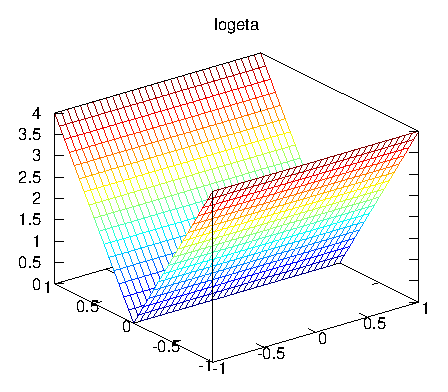
\includegraphics{log_eta_elman_e04_32.eps}} \;
%%   \psfrag{logeta}{$\log_{10} \eta :$ S04}
%%   \resizebox{\imsizes}{!}{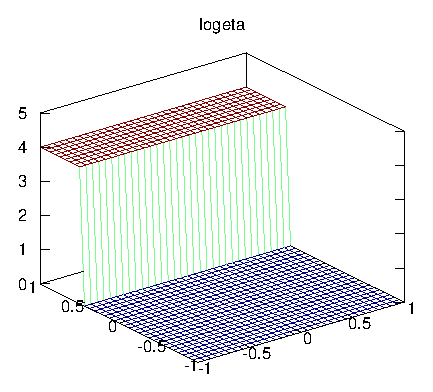
\includegraphics{log_eta_elman_s04_32.eps}} \;
%%   \psfrag{logeta}{$\log_{10} \eta :$ I04}
%%   \resizebox{\imsizes}{!}{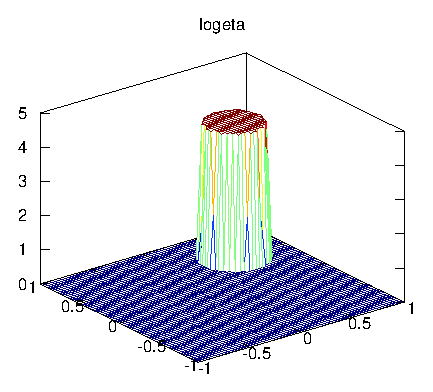
\includegraphics{log_eta_elman_i04_64.eps}} 
%%   \caption{Logarithmic plots of viscosity structures E04, S04, I04}
%%   \label{elm_visc} 
%%\end{figure}
%%
%%Our viscosity models are given entirely as analytic functions, so that iterative
%%solutions of \eqref{Stokes-stab} can be compared with analytic ones.
%%Viscosity steps are represented using the error function:
%%\begin{align}
%%   \mbox{S04:} && \eta &= 5000(\mbox{erf}(1000(y-0.5)+2)+1)+1 \label{S04}\\
%%   \mbox{I04:} && \eta &= 5000(\mbox{erf}(1000(1/16-(x-0.5)^2-(y-0.5)^2)+2)+1)+1 \label{I04}
%%\end{align}
%%The first factor in \eqref{S04} and \eqref{I04} is one half of the viscosity
%%contrast, which is $10^4$ for cases S04 and I04. This convention is extended to
%%$10^8$ and $10^{12}$ for all models and is is indicated by last two digits in
%%the model name. The factor 1000 in \eqref{S04} and \eqref{I04} is chosen as
%%small as possible for the viscosity jump to occur between adjacent grid points
%%also on the finest used grid. There is no loss in generality by setting
%%$\eta_{min} = 1$ as the momentum equation \eqref{mom_weak-final} can always be
%%divided by $\eta_{min}$ together with the calculated pressure. Because
%%\eqref{Stokes-stab} is dominated by the high viscosities in $\mb A$ which also
%%control the size of the residual, the velocities in Examples 1 and 2 are divided
%%by 3, 6 or 9 orders of magnitude, corresponding to the overall viscosity
%%contrast of 4, 8 or 12 orders of magnitude, respectively.
%%
%%The viscosity variations affect the spectral properties of $\mb A$ as expected  
%%(see \tableref{eig-a}). To be spectrally equivalent to the Schur complement,
%%the pressure mass-matrix now also must account for the viscosity variations. Its
%%local contributions are
%%\begin{equation}
%%   m_{e\_{ij}} = \frac{1}{\eta_e} \int_{\Omega_e} \psi_i(x) \psi_j(x) 
%%      \quad \forall \Omega_e \in \mathcal{T}_h
%%   \label{m_local}
%%\end{equation}
%%with viscosity treated as element-wise constant.
%%Eigenvalues of this pressure mass-matrix scaled Schur complement
%%are given in \tableref{eig-var}. They are essentially independent of the 
%%magnitude of the viscosity variation because the reciprocal of $\eta$ is used 
%%in \eqref{c-local} and \eqref{m-local} to build $C$ and $M$.
%%When solving this scaled Schur complement system, the pressure error
%%is minimized in the $M$-norm. To reduce the error in this norm, the iteration
%%number of a Krylov method should be independent of the viscosity variation.
%%To have also the $L_2$-norm of the pressure error reduced below a fixed
%%tolerance, in the worst case the $M$-norm of the error has to be further reduced
%%by the global magnitude of the viscosity variation. This is explored further in
%%\sectionref{stopping}.
%%\begin{table}
%%\caption{Extremal eigenvalues of $\mb A$ for constant and variable viscosity}
%%\label{eig_a}
%%\begin{tabular}{|c|cc|cc|cc|cc|} \hline
%%  &\multicolumn{2}{|c|}{const} & \multicolumn{2}{|c|}{E04} 
%%  & \multicolumn{2}{|c|}{S04} & \multicolumn{2}{|c|}{I04} \\ 
%%  $l$ & $\lambda_{min}$ & $\lambda_{max}$ & $\lambda_{min}$ & $\lambda_{max}$ 
%%   & $\lambda_{min}$ & $\lambda_{max}$ & $\lambda_{min}$ & $\lambda_{max}$ \\ \hline
%%%  $3$ & $0.4356$ & $7.5579$ & $0.2213$ & $1.1219$ & $0.1870$ & $0.6453$ & $0.0119$ & $0.4760$ \\ \hline
%%  $4$ & $0.1120$ & $7.8857$ & $2.2561$ & $23011$ & $0.1534$ & $74758$ & $0.1266$ & $62356$ \\ \hline
%%  $5$ & $0.0282$ & $7.9711$ & $0.5334$ & $36452$ & $0.0371$ & $78488$ & $0.0306$ & $74795$ \\ \hline
%%  $6$ & $0.0071$ & $7.9928$ & $0.1306$ & $48680$ & $0.0091$ & $79601$ & $0.0075$ & $78751$ \\ \hline
%%\end{tabular}
%%\end{table}
%%\begin{table}
%%\caption{Extremal eigenvalues of $M^{-1}(B\mb A^{-1} B + 0.5 C)$ 
%%for variable viscosity}
%%\label{eig-var}
%%\begin{tabular}{|c|cc|cc|cc|cc|} \hline
%%  &\multicolumn{2}{|c|}{E04} & \multicolumn{2}{|c|}{S04} 
%%  & \multicolumn{2}{|c|}{I04} & \multicolumn{2}{|c|}{S12} \\ 
%%  $l$ & $\lambda_{min}$ & $\lambda_{max}$ & $\lambda_{min}$ & $\lambda_{max}$ 
%%   & $\lambda_{min}$ & $\lambda_{max}$ & $\lambda_{min}$ & $\lambda_{max}$ \\ \hline
%%  $4$ & $0.0527$ & $0.8134$ & $0.1676$ & $0.8966$ & $0.0384$ & $0.9240$ & $0.1676$ & $0.8968$ \\ \hline
%%  $5$ & $0.0485$ & $0.8233$ & $0.1674$ & $0.9402$ & $0.0881$ & $0.9633$ & $0.1674$ & $0.9404$ \\ \hline
%%  $6$ & $0.0475$ & $0.8253$ & $0.1659$ & $0.9658$ & $0.1074$ & $0.9829$ & $0.1659$ & $0.9660$ \\ \hline
%%\end{tabular}
%%\end{table}
 
%\bibliographystyle{siam}
%\bibliographystyle{abbrvnat}
\bibliographystyle{wileyj}
%\bibliographystyle{plainnat}
%\bibliographystyle{spphys}
\bibliography{wz,ck,literatur} %(wz must be read first since it contains definitions)

\end{document} 

